\documentclass[12pt, letterpaper, twoside]{article}
\usepackage[utf8]{inputenc}

\usepackage{geometry}
\usepackage{algorithm}
\usepackage{algpseudocode}
\usepackage[backend=bibtex,style=verbose-trad2]{biblatex}
\usepackage{csquotes}
\usepackage{amssymb}
\usepackage{amsmath}
\usepackage{multicol}
\usepackage{graphicx}
\usepackage{float}

\setlength{\parskip}{1em}
\bibliography{citation-13218946.bib}
\bibliography{PMC3588402.bib}
\bibliography{10.1007_F3-540-48017-X_15.bib}

\title{Solucionando el problema de la mochila en el Modelo Sticker}
\author{Ernesto Mancebo}
\date{Febrero 2020}

\usepackage{tikz}

\begin{document}
    \maketitle
    \begin{abstract}
        Este artículo es un estudio del paper \emph{Solving Knapsack Problems in a Sticker Based Model} de los profesores Mario P{\'e}rez-Jim{\'e}nez y Fernando Sancho-Caparrini\autocite{ref10.1007/3-540-48017-X_15}, el cual tiene como objetivo la resolución de los problema \emph{suma de subconjuntos} y \emph{porblema de la mochila}, para éste último en sus versiones acotada y la no acotada, utilizando como apoyo para la resolución de ambos problemas las subrutinas \emph{ordenado por cardinalidad} y \emph{llenado en paralelo}.
    \end{abstract}

    \newpage
    \tableofcontents

    \newpage
    \section{Modelo Sticker}
    El Modelo Sticker es un modelo de computación inpirado en cadenas de ADN propuesto por Sam Roweis \autocite{sticker_model}, donde tal modelo se basa en procedimientos de filtrado, con memoria de acceso aleatorio y una nueva manera de codificar la información. En ese mismo orden, éste modelo se distingue de otros modelos computacionales por la última característica enlistada, la manera en que codifica la información.

    \subsection{Concepto de Cadena de Memoria}
    El eje central de este modelo son las cadenas de memoria, tales cadenas consisten en hebras simples de ADN del tipo $(n, k, m)$, tal que $n\geq k.m$, siendo $n$ la longitud de la cadena, $k$ las cantidad de subcadenas o regiones, y $m$ la longitud de cada subcadena.

    Asimismo, un sticker es un elemento asociado a una región en la cadena de memoria, una vez asociado se dice que la región está complementada, transformando la cadena en una hebra doble parcial. En ese sentido, se dice que en cada región donde haya un sticker complementándole, esta región está \emph{activada}, mientras que la región donde se carezca de sticker se dice está \emph{desactivada}. Tal abstracción binaria también se puede expresar de modo \emph{0/1}.

    \newpage
    \begin{figure}[h!]
        \centering
        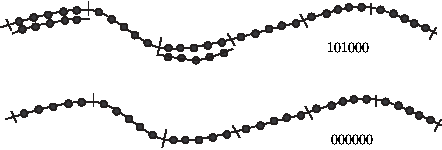
\includegraphics[width=\linewidth]{sticker.png}
        \caption{Cadenas de Memoria}
    \end{figure}

    En esta imágen se ilustran dos cadenas de memoria, la primera cadena de memoria tiene un sticker en la primera y tercera región, por lo que estas están \emph{activadas}, leyéndose $101000$; mientras que para la segunda cadena de memoria no existe sticker alguno asociado, por ello todas las regiones están \emph{desactivadas}, leyéndose $000000$.

    \subsection{Concepto de Tubo}
    Dentro del modelo sticker un tubo consiste en un multiconjunto cuyo contenido son complejos de memorias del mismo tipo.

    Las operaciones principales a ser realizadas sobre un tubo son:
    \begin{itemize}
        \item \emph{mezclar}$(T_1,T_2)$: Retorna la unión de los dos tubos devolviendo un solo tubo el cual contiene cada complejo de memoria proveniente de ambos tubos. También se nota como $(T_1\cup T_2)$.
        \item \emph{separar}$(T, i)$: Para un tubo $T$ y un índice $i$ tal que $(1 \leq i \leq n)$, retorna un $+(T, i)$ y $-(T, i)$, de modo que el primer tubo contiene todos los complejos de memoria cuya región $i$-ésima esté \emph{activada}, mientras que el segundo contiene los complejos cuya región $i$-ésima \emph{desactivada}.
        \item \emph{encender}$(T, i)$: Para un tubo $T$ y un índice $i$ tal que $(1 \leq i \leq n)$, retorna un tubo $T'$ con la región $i$-ésima \emph{activada} en cada complejo de memoria.
        \item \emph{apagar}$(T, i)$: Para un tubo $T$ y un índice $i$ tal que $(1 \leq i \leq n)$, retorna un tubo $T'$ con la región $i$-ésima \emph{desactivada} en cada complejo de memoria.
        \item \emph{leer}$(T)$: Dado un tubo $T\neq\emptyset$, lee su contenido.
    \end{itemize}
    \subsection{Concepto de Librería}
    Una librería dentro del modelo sticker consiste en complejos de memoria de modo $(k,l)$, teniendo $k$ sub cadenas y las primeras $l$ subcadenas están \emph{activadas} o \emph{desactivadas} en todas sus posibles combinaciones, mientras que las regiones $k -l$ restantes están \emph{desactivadas}\autocite{Taghipour2013}.

    \begin{figure}[h!]
        \centering
        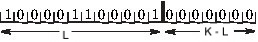
\includegraphics[]{libreria.jpg}
        \caption{Librería$(k,l)$}
    \end{figure}

    \section{Subrutina Ordenado por Cardinalidad}
    \textbf{Problema:} Sea $A = \{1,\dots,p\}$, $B = \{b_1,\dots,b_s\} \subseteq A$, $\mathcal{F} = \{D_1,\dots,D_t\} \subseteq \mathcal{P}(A)$. Ordene los conjuntos de $\mathcal{F}$ de acuerdo a su cardinalidad en $B$, o en otras palabras, la cantidad de elementos de $B\cap D_i$.


    El paper bajo estudio nos sugiere el implementar un programa molecular definido con las siguientes características:
    \begin{itemize}
        \item  La entrada será un tubo $T_0$ conteniendo complejos de memoría codificando cada conjunto de la familia $\mathcal{F}$. Para esto, cada complejo de memoria en $T_0$ se representará mediante la función booleana  $T_0=\{\{\sigma:|\sigma|=p\;\land\;\exists{j}\;(\chi_{D_j}=\sigma)\}\}$; tal que $\chi_{D_j}$ es la función característica de $D_j$ en $A$, siendo $(\chi_{D_j}(i) = 1$ si $i \in D_j$ de lo contrario $\chi_{D_j}(i) = 0$ si $i \in A - D_j)$.
        \item  El programa consistirá en un bucle principal realizando $s$ pasos, donde para el paso $i$-ésimo se tendrá $i+1$ tubos $(T_0, T_1,\dots,T_i)$, tales tubos generados verificando la condición $\forall\sigma\;(\sigma\in T_j \rightarrow|\sigma\cap\{b_1,\dots,b_i\}|=j)$. Los tubos se compondrán de la siguiente manera:
        \begin{equation*}
            \begin{cases}
                T_0=-(T_0,b_{i+1}) \\
                T_j=+(T_{j-1}, b_{i+1}) \cup -(T_j, b_{i+1}) \quad (1\leq{j}\leq{i}) \\
                T_{i+1} = +(T_i,b_{i+1})
            \end{cases}
        \end{equation*}
    \end{itemize}

    \subsection{Algoritmo}
    Las ideas previas nos indican el siguiente algoritmo: 
    \begin{algorithm}
        \begin{algorithmic}[1]
            \Procedure{$Cardinal\_Sort$}{$T_0,B$}
                \For { $i=1$ to $s$ }
                    \State $(T_0, T'_0) \leftarrow separar(T_0, b_i)$
                    \For { $j=0$ to $i-1$ }
                        \State {$(T'_{j+1},T''_j) \leftarrow separar(T_j,b_i)$}
                        \State {$T_j \leftarrow mezclar(T'_j,T''_j)$}
                    \EndFor
                    \State {$T_i \leftarrow T'_i$}
                \EndFor
                \State \textbf{return} $T_0,\dots,T_s$
            \EndProcedure
        \end{algorithmic}
    \end{algorithm}

    \newpage
    \subsection{Otras Notaciones}
    Para usos posteriores dentro de este informe, podemos notar el uso de \emph{Cardinal\_Sort} de modo:
    \begin{itemize}
        \item $Cardinal\_Sort(T_0)$ cuando $B=A$.
        \item $Cardinal\_Sort(T_0, l, k)$ cuando $B=\{l, l+1,\dots,k\}$.
    \end{itemize}

    \subsection{Proposiciones}
    \subsubsection{Proposición 1}
    $\forall{i}\;(1\leq{i}\leq{s}\rightarrow\forall{j}\leq{i}\;\forall{\sigma}(\sigma\in{T_{i,j}}\rightarrow|\sigma\cap{B_i}|=j))$.

    \emph{Prueba}. Por inducción en $i$, veamos que $\forall{j}\leq{1}$ $\forall\sigma\in{T_{1,j}}(|\sigma\cap{B_1}|=j)$.
    \begin{itemize}
        \item Sea $\sigma\in{T_{1,0}} = +(T_{0,-1}, b_1) \cup -(T_{0,0}, b_1).$ Partiendo de que $T_{0,-1}=\emptyset$ y $T_{0,0}=T_0$, resultando que $\sigma\in{-(T_0,b_1)}$; esto es, $b_1\notin\sigma$; por lo que $|\sigma\cap{B_1}|=0$.
        \item Sea $\sigma\in{T_{1,1}} = +(T_{0,0}, b_1) \cup -(T_{0,1}, b_1).$ Partiendo de que $T_{0,1}=\emptyset$ y $T_{0,0}=T_0$, resultando que $\sigma\in{-T_{0,0}}=T_0$ y $b_1\in\sigma$; por lo que $|\sigma\cap{B_1}|=1$.
    \end{itemize}

    Sea $i (1\leq{i}<s)$ tal que $\forall{j}\leq{i}$ $\forall\sigma\in{T_{i,j}}(|\sigma\cap{B_i}|=j)$. Veamos que el resultado verifica que para $i+1$. Por ello, se procede por inducción en $j$: $\forall{j}\leq{i+1}$ $\forall\sigma\in{T_{i+1, j}}\;(|\sigma\cap{B_{i+1}}|=j)$.
    \begin{itemize}
        \item Sea $\sigma\in{T_{i+1, 0}}=+(T_{i, -1}, b_{i+1})\cup-(T_{i,0},b_{i+1})$. Siendo $T_{i,-1}=\emptyset$, resulta que $\sigma\in{T_{i,0}}$ y $b_{i+1}\notin\sigma$, por hipótesis de inducción deducimos que $|\sigma\cap{B_i}|=0$. Por lo que $|\sigma\cap{B_{i+1}}|=1$, partiendo de que $b_{i+1}\notin\sigma$.
        \item Sea $j>0$ y $\sigma\in{T_{i+1,j}}=+(T_{i,j-1}, b_{i+1})\cup-(T_{i,j},b_{i,-1})$, entonces:
        \begin{itemize}
            \item Si $\sigma\in{T_{i,j}}$ y $b_{i+1}\in\sigma$, por hipótesis de inducción tenemos que $|\sigma\cap{B_i}|=j-1$. Partiendo de que $b_{i+1}\in\sigma$, se concluye en que $|\sigma\cap{B_{i+1}}|=j-1+1=j$.
            \item Si $\sigma\in{T_{i,j}}$ y $b_{i,j}\notin\sigma$, por hipótesis de inducción tenemos que $|\sigma\cap{B_i}|=j$. Tal que $b_{i+1}\notin\sigma$, tenemos que $|\sigma\cap{B_{i+1}}|=j$.
        \end{itemize}
    \end{itemize}
    \subsubsection{Proposición 2}
    $\forall\sigma\in{T_0}\;\forall{i}\;(0\leq{i}\leq{s}\rightarrow\sigma\in{T_{i,|\sigma\cap{B_i}|}})$


    \emph{Prueba}. Por indución en $i$. Para $i=0$, el resultado toca la trivialidad. Asumimos que el resultado mantiene que para $i\;(0\leq{i}<s)$, se comprueba esto para $i+1$.
    \begin{itemize}
        \item Si $b_{i+1}\in\sigma$, tenemos que $|\sigma\cap{B_{i+1}}|=1 + |\sigma\cap{B_i}|$. Por hipótesis de inducción, $\sigma\in{T_{i,|\sigma\cap{B_{i+1}|}}}$, entonces $\sigma\in{+(T_{i,|\sigma\cap{B_i}|,b_{i+1}})}\subseteq{T_{i+1,|\sigma\cap{B_i}|+1}}$.
        \item Si $b_{i+1}\notin\sigma$, entonces $|\sigma\cap{B_{i+1}}|=|\sigma\cap{B_i}|$. Por hipótesis de inducción $\sigma\in{T_{i, |\sigma\cap{B_i}|}}$, entonces $\sigma\in{-(T_{i,|\sigma\cap{B_i}|, b_{i+1}})}$ $\subseteq{T_{i+1, |\sigma\cap{B_i}|}}=T_{i+1, |\sigma\cap{B_{i+1}}|}$.
    \end{itemize}
    \subsection{Corolarios}

    \subsubsection{Corolario 1 - Robustez del Algoritmo}
    Si $\forall{j}\;\forall\sigma\;(0\leq j \leq s \land \sigma\in T_{s,j} \rightarrow |\sigma\cap B| = j)$. Dicho de otra manera, $j$ debe de ser un valor entre $0$ y $s$, y para cada complejo de memoria $\sigma$ existente en $T_{s,j}$, tantas moléculas contenga para la cardinalidad $|\sigma\cap B|$,esta será igual a $j$. 
    \subsubsection{Corolario 2 - Completitud del Algoritmo}
    Si $\sigma\in T_0$ y $|\sigma\cap B| = j$, entonces $\sigma\in T_{s,j}$. Esto es, si existe un complejo de memoria en el tubo de entrada, y la cardinalidad de la misma en $B$ es $j$, pues el mismo complejo de memoria debe de aparecer en el tubo $j$-ésimo.

    \newpage
    \subsection{Traza Subrutina Ordenado por Cardinalidad}
    A modo de ilustrar el comportamiendo y los conceptos empleados en el algoritmo concebido, tenemos:
    \begin{itemize}
        \item $A: \{0, 1, 2, 3, 4, 5, 6\}$
        \item $B: \{1, 2, 4\}$
        \item $\mathcal{F}: \{\{2, 6\}, \{3\}, \{4\}, \{2, 4\}\}$
    \end{itemize}
    Identificando los elementos que cumplen $B\cap D_j$ en $\mathcal{F}$ le resaltamos en rojo de modo que tenemos: $\{\{\textcolor{red}{2}, 6\}, \{3\}, \{\textcolor{red}{4}\}, \{\textcolor{red}{2, 4}\}\}$. Codificando $\mathcal{F}$ para llevarlo a un tubo tendíamos: 


    $
        \begin{bmatrix}
            0\,0\,1\,0\,0\,0\,1 \\
            0\,0\,0\,1\,0\,0\,0 \\
            0\,0\,0\,0\,1\,0\,0 \\
            0\,0\,1\,0\,1\,0\,0 \\
        \end{bmatrix}
    $ 


    Este $T_0$ codificando $\mathcal{F}$ tras la ejecución de \emph{Cardinal\_Sort} tendremos: 

        $
        \begin{array}{l}
            T_0: [\,0\,0\,0\,1\,0\,0\,0\,] \\
            T_1: \left[\begin{array}{l} 0\,0\,0\,0\,1\,0\,0 \\ 0\,0\,1\,0\,0\,0\,1 \end{array} \right] \\
            T_2: [\,0\,0\,1\,0\,1\,0\,0\,] \\
            T_3: [] \\
            T_4: [] \\
            T_5: [] \\
            T_6: [] 
        \end{array}
        $ 


    Cumpliendo de esta manera los corolarios 1 y 2.

    \newpage
    \section{Subrutina de Llenado}
    Sea $A=\{1,\dots,p\}$, $r \in \mathbb{N}$ y $f:A\rightarrow\mathbb{N}$ una función. Si $B\subseteq A$, notamos $f(B)=\sum_{i\in B}f(i)$, por conveniencia deifnimos que para $f(0)=0$. Sea $q_f=f(A)$, $A_i=\{0,\dots,i\}$ $(0\leq i\leq p)$, y $T_0$ un multiconjunto de complejos de memoria de forma $(n,k,m)$ con $k\geq p+r+q_f$.


    Si $\sigma\in T_0$, podemos asumir que tal complejo de memoria está formado por las regiones:
    \begin{multicols}{2}
        \begin{itemize}
            \item $(A\sigma )=\sigma (1)\dots\sigma (p)$
            \item $(L\sigma )=\sigma (p+1)\dots\sigma (p+r)$
            \item $(F\sigma)=\sigma(p+r+1)\dots\sigma(p+r+q_f)$
            \item $(R\sigma)=\sigma(p+r+q_f+1)\dots$
        \end{itemize} 
    \end{multicols}


    La subrutina opera sobre $T_0$ modificando sus elemento haciendo las moléculas del tubo de salida en $(F_\sigma)$ el peso con respecto a $f$ del subconjunto en $A$ codificado en $(A_\sigma)$, mientras que las zonas $(R_\sigma)$ y $(L_\sigma)$ no son modificadas, expresándose todo esto de forma:

        \begin{equation*}
            \begin{aligned}
                \sum_{i=1}^{p}\sigma(i)f(i) \qquad \sum_{j=p+r+1}^{p+r+q_f}\sigma(j)
            \end{aligned}
        \end{equation*}

    \subsection{Algoritmo}
    \begin{algorithm}
        \begin{algorithmic}[1]
            \Procedure{$Parallel\_Fill$}{$T_0,f,p,r$}
            \For { $i=1$ to $p$ }
                \State $(T^+, T^-) \leftarrow separar(T_{0}, i)$
                \For { $j=1$ to $f(i)$ }
                    \State {$T^+ \leftarrow encender(T^+,p+r+f(A_{i-1})+j)$}
                \EndFor
                \State {$T_0 \leftarrow mezclar(T^+, T^-)$}
            \EndFor
            \State \textbf{return} $T_0$
            \EndProcedure
        \end{algorithmic}
    \end{algorithm}

    Para cada $i\;(1\leq i \leq p)$ se consiredan las regiones: $R_i=\{p+r+f(A_{i-1})+1,\dots,p+r+f(A_i)\}$.

    \subsection{Lemas}
    \subsubsection{Lema 1}
    \begin{enumerate}
        \item La zona inicial de la molécula (codificando el subconjunto de $A$) no cambia durante la ejecución del programa, siendo esto:
        \begin{equation}
            \begin{aligned}
                \forall\sigma\in{T_0}\;\forall{k}\;(1\leq{k}\leq{p}\rightarrow{A\sigma}=(A\sigma^{k}))
            \end{aligned}
        \end{equation}
        \item Las moléculas que son obtenidas in el $k$-ésimo paso del búcle principal es almacenado en el tubo $T_k$, siendo esto:
        \begin{equation}
            \begin{aligned}
                \forall\sigma\in{T_0}\;\forall{k}\;(1\leq{k}\leq{p}\rightarrow\sigma^{k}\in{T_k})
            \end{aligned}
        \end{equation}
        \item Cada molécula en el $k$-ésimo tubo proviene de alguna molécula del tubo inicial, siendo esto:
        \begin{equation}
            \begin{aligned}
                \forall{k}\;(1\leq{k}\leq{p}\rightarrow\forall\tau\in{T_k}\;\exists\sigma\in{T_0}(\sigma^k=\tau))
            \end{aligned}
        \end{equation}
        \item La ejecución de un paso en el bucle principal no modifica las regiones correspondiente a los pasos previos, siento esto:
        \begin{equation}
            \begin{aligned}
                \forall\sigma\in{T_0}\;\forall{i}\;\forall{k}\;(1\leq{i}\leq{k}\leq{p}\rightarrow\sigma^{i}_{|R_i}=\sigma^{k}_{|R_i})
            \end{aligned}
        \end{equation}
        \item Luego de la ejecución del $i$-ésimo paso del bucle principal, la región $R_i$ en $\sigma$ ha sido modificada para de acuerdo con el valor de $\sigma(i)$, siendo esto:
        \begin{equation}
            \begin{aligned}
                \forall\sigma\in{T_0}\;\forall{i}\;\forall{k}\;(1\leq{i}\leq{k}\leq{p}\rightarrow\sigma^{k}_{|R_i}\equiv\sigma(i))
            \end{aligned}
        \end{equation}
        \item La ejecución de un paso en el bucle principal no altera las zonas $(L\sigma)$ ni $(R\sigma)$, siendo esto:
        \begin{equation}
            \begin{aligned}
                \forall\sigma\in{T_0}\;\forall{k}\;(1\leq{k}\leq{p}\rightarrow(L\sigma)=(L\sigma^{k})\land(R\sigma)=(R\sigma^{k}))
            \end{aligned}
        \end{equation}
    \end{enumerate}

    Lo resultante para estos lemas nos aseguran que el bucle principal modifique exclusivamente la región $R_i$ en una molécula, codificando de esta manera el peso para cada una de estas.

    \subsection{Proposiciones}
    \subsubsection{Proposición 3}
    Sea $B\subseteq{A}$ tal que $\sigma_{B}\in{T_0}$, entonces para cada $k\;(1\leq{k}\leq{p})$, tenemos que:
    \begin{equation*}
        f(B\cap{\{1,\dots,k\}})=\sum^{p+r+f(A_k)}_{j=p+r+1}=\sigma^{k}_{B}(j)
    \end{equation*}
    \emph{Prueba}. Partiendo de $(1)$ se tiene que
    \begin{equation*}
        f(B\cap{\{1,\dots,{k}\}})=\sum^{k}_{i=1}f(i).\sigma_{B}(i)=\sum^{k}_{i=1}f(i).\sigma^{k}_{B}(i)
    \end{equation*}
    Por otro lado, $(1)$ y $(5)$ asegura que:
    \begin{equation*}
        f(i).\sigma^{k}_{B}(i)=\sum_{j\in{R_{i}}}\sigma^{k}_{B}(j)\;(1\leq{i}\leq{k})
    \end{equation*}
    \subsection{Corolarios}
    \subsubsection{Corolario 3}
    Para cada $B\subseteq{A}$ tal que $\sigma_{B}\in{T_0}$ existe algún $\tau\in{T_{p}}$ tal que $f(B)=\sum^{p+r+q_f}_{i=p+r+1}\tau(i)$.

    \emph{Prueba}. Dado un $B\subseteq{A}$, consideremos que la molécula asociada $\sigma_{B}\in{T_0}$. Ello satisface el considerar $\tau=\sigma^{p}_{B}$, partiendo de que $f(B)=f(B\cap{\{1,\dots,p\}})=\sum^{p+r+q_f}_{j=p+r+1}\sigma^{p}_{B}(j)$. 

    \newpage
    \subsection{Traza Subrutina de Llenado}
    A fin de ilustrar el comportamiento para el algoritmo bajo estudio, tenemos:
    \begin{multicols}{2}
        \begin{itemize}
        \item $A: \{1, 2, 3, 4\}$
        \item $B: \{1, 2, 4\}$
        \item $T_0: \{\{1,2,3\}, \{1\}, \{2,3,4\}\}$
        \item $p = 4$
        \item $r = 1$
        \item $q_f= 20$
        \end{itemize}
    \end{multicols}

    Definido lo previo, tendremos las siguientes zonas delimitadas de la siguiente manera:
    \begin{multicols}{2}
        \begin{itemize}
            \item $(A\sigma )=\sigma (1)\dots\sigma (4)$
            \item $(L\sigma )=\sigma (4+1)\dots\sigma (4+1)$
            \item $(F\sigma)=\sigma(4+1+1)\dots\sigma(4+1+20)$
            \item $(R\sigma)=\sigma(4+1+20+1)\dots$
        \end{itemize} 
    \end{multicols}

    Para el tubo $T_0$ los valores que cumplen $B\cap{A}$ le resaltamos en rojo, teniendo $T_0: \{\{\textcolor{red}{1, 2}, 3\}, \{\textcolor{red}{1}\}, \{\textcolor{red}{2},3,\textcolor{red}{4}\}\}$, donde al codificar este con las delimitaciones previas, tenemos:


        $
            \begin{bmatrix}
                \textcolor{red}{1\,1\,1\,0}\textcolor{teal}{\,0}\,0\,0\,0\,0\,0\,0\,0\,0\,0\,0\,0\,0\,0\,0\,0\,0\,0\,0\,0\,0\\
                \textcolor{red}{1\,0\,0\,0}\textcolor{teal}{\,0}\,0\,0\,0\,0\,0\,0\,0\,0\,0\,0\,0\,0\,0\,0\,0\,0\,0\,0\,0\,0 \\
                \textcolor{red}{0\,1\,1\,1}\textcolor{teal}{\,0}\,0\,0\,0\,0\,0\,0\,0\,0\,0\,0\,0\,0\,0\,0\,0\,0\,0\,0\,0\,0
            \end{bmatrix}
        $


Nótese que que la región $(A_\sigma)$ y $(L_\sigma)$ se han resaltado para su apreciación, mientras que lo restante se reserva para la región $(F_\sigma)$.


Una vez odificado el tubo $T_0$, éste al ser procesado por $Parallel\_Fill$, tendremos como salida un tubo de la siguiente manera:


    $
        \begin{bmatrix}
            \textcolor{red}{1\,1\,1\,0}\textcolor{teal}{\,0}\,1\,1\,1\,1\,0\,0\,0\,0\,0\,0\,0\,0\,0\,0\,0\,0\,0\,0\,0\,0\\
            \textcolor{red}{1\,0\,0\,0}\textcolor{teal}{\,0}\,1\,0\,0\,0\,0\,0\,0\,0\,0\,0\,0\,0\,0\,0\,0\,0\,0\,0\,0\,0 \\
            \textcolor{red}{0\,1\,1\,1}\textcolor{teal}{\,0}\,1\,1\,1\,1\,1\,1\,1\,1\,1\,1\,1\,1\,1\,0\,0\,0\,0\,0\,0\,0
        \end{bmatrix}
    $


    \newpage
    \section{Problema de Suma de Subconjuntos}
    \textbf{Problema:} Sea $A=\{1,\dots,p\}$ y $\omega\rightarrow\mathbb{N}$ una función peso. Sea $k\in\mathbb{N}$, tal que $k\leq\omega(A)=q_\omega$, determinar si existe un subconjunto $B\subseteq A$, tal que la suma de los pesos en $B$ sea exactamente $k$.


    Definido una vez el problema, el paper bajo estudio presenta un diseño de un programa dentro del modelo sticker tal que resuelve el problema de la suma de subcojnuntos. El tubo de entrada $T_0$ conteniendo una librería de forma $(p+q_\omega, q)$. 


    La primera fase, la fase de llenado, cada molécula $\sigma$ del tubo de entrada será llenado a fin de conseguir en los últimos componentes $q$ el peso de los subcojnuntos que codifica. Los tubos obtenidos luego serán ordenados de acuerdo a su cardinalidad. Por último, el tubo $k$-ésimo es leído, donde tal tubo $T_k$ representa el peso buscado.


    \subsection{Algoritmo}
    La descripción del planteamiento explicado sugiere un programa molecular como el que sigue:
    \begin{algorithm}
        \begin{algorithmic}[1]
            \Procedure{$Subset\_Sum$}{$p,w,k$}
            \State {$q_w \leftarrow \sum_{i=1}^{p}w(i)$}
            \State {$T_0 \leftarrow $ Libería$(p+q_w,p)$}
            \State {$T_1 \leftarrow Parallel\_Fill(T_0,w,p,0)$}
            \State {$T_{salida} \leftarrow Cardinal\_Sort(T_1,p+1,p+q_w)[k]$}
            \State{$leer(T_{salida})$}
            \EndProcedure
        \end{algorithmic}
    \end{algorithm}

    \subsection{Diseño}

    La implementación del algoritmo expuesto considera el uso de $4+2q$ tubos $T$ y un coste de $2p+q+1+\frac{q.(q+3)}{2}$ operaciones o pasos. Asimismo, el diseño de éste programa no sólo soluciona un problema de desición pues a su vez retorna todas las soluciones posibles al problema propuesto.

    \subsection{Teoremas}
    \subsubsection{Theorema 1 - Robustez}
    Si $T_{salida}\neq\emptyset$, entonces existe un $B\subseteq{A}$ tal que $\omega(B)=k$.

    \emph{Prueba}. Tomando $\tau\in{T_{salida}}$, aplicando $(3)$ y la proposición 3, obtenemos $\sigma\in{T_0}$ verificamos que el resultado para $B_\sigma$.

    \subsubsection{Theorema 2 - Completitud}
    Sea $\sigma\in{T_0}$ tal que $\omega(B_\sigma)=k$, entonces $T_{salida}\neq\emptyset$.

    \emph{Prueba}. Sea $\sigma\in{T_0}$ tal qeu $\omega(B_\sigma)=k$, partiendo del corolario 3, luego de la ejecución de la subrutina de llenado, tenemos una molécula $\tau=\sigma^{p}\in{T_1}$ tal que $\omega(B_\sigma)=\sum^{p+q_\omega}_{i=p+1}\tau(i)$, entonces $\tau\in{T_{salida}}$.

    \newpage
    \subsection{Traza}
    A fin de ilustrar el comportamiento para el algoritmo bajo estudio y tomando como referencia el tubo del apartado anterior $T_0$ para simplicitud, tenemos:
    \begin{multicols}{2}
        \begin{itemize}
        \item $A: \{1, 2, 3, 4\}$
        \item $B: \{1, 2, 4\}$
        \item $T_0: \{\{1,2,3\}, \{1\}, \{2,3,4\}\}$
        \item $p = 4$
        \item $r = 1$
        \item $q_f= 20$
        \item $k =4$
        \end{itemize}
    \end{multicols}


    Una vez definido el tubo $T_0$, y éste procesado por $Parallel\_Fill$, tendríamos como salida el tubo $T_1$ codificado de la siguiente manera:

    $
        \begin{bmatrix}
            \textcolor{red}{1\,1\,1\,0}\textcolor{teal}{\,0}\,1\,1\,1\,1\,0\,0\,0\,0\,0\,0\,0\,0\,0\,0\,0\,0\,0\,0\,0\,0\\
            \textcolor{red}{1\,0\,0\,0}\textcolor{teal}{\,0}\,1\,0\,0\,0\,0\,0\,0\,0\,0\,0\,0\,0\,0\,0\,0\,0\,0\,0\,0\,0 \\
            \textcolor{red}{0\,1\,1\,1}\textcolor{teal}{\,0}\,1\,1\,1\,1\,1\,1\,1\,1\,1\,1\,1\,1\,1\,0\,0\,0\,0\,0\,0\,0
        \end{bmatrix}
    $


    Este tubo $T_1$, una vez ordenado por $Cardinal\_Sort$ resultaría de la siguiente manera:

    $
    \begin{array}{l}
        T_0: [\;] \\
        T_1: [\;\textcolor{red}{1\,0\,0\,0}\textcolor{teal}{\,0}\,1\,0\,0\,0\,0\,0\,0\,0\,0\,0\,0\,0\,0\,0\,0\,0\,0\,0\,0\,0\;] \\
        T_2: [\;] \\
        T_3: [\;] \\
        T_4: [\;\textcolor{red}{1\,1\,1\,0}\textcolor{teal}{\,0}\,1\,1\,1\,1\,0\,0\,0\,0\,0\,0\,0\,0\,0\,0\,0\,0\,0\,0\,0\,0\;] \\
        T_5: [\;] \\
        T_6: [\;] \\
        \dots \\
        T_{13}: [\;\textcolor{red}{0\,1\,1\,1}\textcolor{teal}{\,0}\,1\,1\,1\,1\,1\,1\,1\,1\,1\,1\,1\,1\,1\,0\,0\,0\,0\,0\,0\,0\;] \\
        \dots
    \end{array}
    $ 


    Finalmente, para un $k=4$, el tubo a buscar es el $T_4$, por lo que tendríamos como salida: $\textcolor{red}{1\,1\,1\,0}\textcolor{teal}{\,0}\,1\,1\,1\,1\,0\,0\,0\,0\,0\,0\,0\,0\,0\,0\,0\,0\,0\,0\,0\,0$; de modo que éste resultado da cumpliento  con los teoremas 1 y 2.


    \newpage
    \section{Problema de la Mochila Acotado}
    \textbf{Problema:} sea $A=\{1,\dots,p\}$ un conjunto finito no vacío, $\omega:A\rightarrow\mathbb{N}$ una función peso y $\rho:A\rightarrow\mathbb{N}$ una función valor. Sea $k, k'\in\mathbb{N}$ tal que $k\leq\omega(A)=q_\omega$ y $k'\leq\rho(A)=q_\rho$; determine si existe un subconjunto $B\subseteq A$ tal que $\omega(B)\leq k$ y $\rho(B)\geq k'$.


    Esto nos lleva plantear el diseño de un programa molecular el cual resuelva el problema propuesto utilizando una librería$(p+q_\omega+q_\rho, p)$.


    En la fase inicial, la fase de llenado, se procede como en el problema previo: cada complejo de memoria en el tubo inicial es llenado apropiadamente tal que codifique el \emph{peso} asociado al subconjunto, seguido de la ordenación de los mismos de acuerdo a su cardinalidad de $\omega(A\sigma)$, empezando por obtener algunos tubos $T_0,\dots,T_{q_\omega}$ tales que $\forall\sigma\;(\sigma\in T_j \Rightarrow |\omega(A\sigma)|=j)$.


    Con los tubos $T_0\cup\dots\cup T_k$ se lleva a cabo una segunda operación de llenado, esta con respecto a los \emph{valores}. Posteriormente, las moléculas $\sigma$ del tubo resultante son ordenadas con respecto a su cardinalidad en $\rho(A\sigma)$ , obteniendo nuevamente una serie de tubos de forma $T_0,\dots,T_{q_\rho}$, tales que $\forall\sigma\;(\sigma\in T_j \Rightarrow |\rho(A\sigma)| = j)$.


    Finalmente, se obtiene la solución al problema con tubos $T_{k'}\cup\dots T_{q_\rho}$ y estos son leidos.
    \newpage
    \subsection{Algoritmo}
    Las directrices del apartado anterior guían a definir un programa molecular de la siguiente forma

    \begin{algorithm}
        \begin{algorithmic}[1]
            \Procedure{$Bounded\_Knapsack$}{$p,w,\rho,k,k'$}
            \State {$q_w \leftarrow \sum_{i=1}^{p}w(i);\, q_\rho \leftarrow \sum_{i=1}^{p}\rho(i);\, T_0 \leftarrow $Libería$(p+q_w+q_\rho,p)$}
            \State {$T_0 \leftarrow Parallel\_Fill(T_0,w,p,0)$}
            \State {$T_0 \leftarrow Cardinal\_Sort(T_0,p+1,p+q_w)$}
            \State {$T_1 \leftarrow \emptyset$}
            \For {$i=1$ to $k$}
                \State {$T_1 \leftarrow mezclar(T_1,Cardinal\_Sort(T_0,p+1,p+q_w)[i])$}
            \EndFor
            \State {$T_0 \leftarrow Parallel\_Fill(T_1,\rho,p,q_w)$}
            \State {$Cardinal\_Sort(T_0,p+q_w+1,p+q_w,q_\rho)$}
            \State {$T_1 \leftarrow \emptyset$}
            \For {$i=k'$ to $q_\rho$}
                \State {$T_1 \leftarrow merge(T_1,Cardinal\_Sort(T_0,p+q_w + 1,p+q_w+q_\rho)[i])$}
            \EndFor
            \State{$leer(T_1)$}
            \EndProcedure
        \end{algorithmic}
    \end{algorithm}
    \newpage
    \subsection{Diseño}
    \newpage
    \section{Problema de la Mochila No Acotado}
    \textbf{Problema:} bajo las mismas condiciones del problema anterior, determinar si un subconjunto $B\subseteq A$ tal que $\rho(B) =max\{\rho(C):C\subseteq A\;\land\;\omega(C) \leq k\}$.


    Una solución molecular es obtenida a partir del problema la mochila acotado, mas un cambio en la fase final en donde se ordenan los tubos de salida con respecto a su valor y se elige sólamente el tubo con mayor valor.

    \subsection{Algoritmo}
    La nueva propuesta lleva a considerar un programa molecular similar al previo mas se ha de notar las variaciones en la salida del programa al retornar sólo el tubo con mayor valor.
    \begin{algorithm}
        \begin{algorithmic}[1]
            \Procedure{$Unbounded\_Knapsack$}{$p,w,\rho,k,k'$}
            \State {$q_w \leftarrow \sum_{i=1}^{p}w(i);\,q_\rho \leftarrow \sum_{i=1}^{p}\rho(i);\, T_0 \leftarrow $Libería$(p+q_w+q_\rho,p)$}
            \State {$T_0 \leftarrow Parallel\_Fill(T_0,w,p,0)$}
            \State {$T_0 \leftarrow Cardinal\_Sort(T_0,p+1,p+q_w)$}
            \State {$T_1 \leftarrow \emptyset$}
            \For {$i=1$ to $k$}
            \State {$T_1  \leftarrow  mezclar(T_1,Cardinal\_Sort(T_0,p+1,p+q_w)[i])$}
            \EndFor
            \State {$T_0 \leftarrow Parallel\_Fill(T_1,\rho,p,q_w)$}
            \State {$i\leftarrow{q_\rho};t\leftarrow{0}$}
            \While {$i \geq 1\;\land\;t==0$}
                \State {$T' \leftarrow Cardinal\_Sort(T_0,p+q_w +1,p+q_w+q_\rho)[i]$}
                \If{$T'\neq\emptyset$}
                    \State{$leer(T')$}
                    \State{$t\leftarrow{1}$}
                \Else
                    \State{$i\leftarrow{i-1}$}
                \EndIf
            \EndWhile
            \EndProcedure
        \end{algorithmic}
    \end{algorithm}
    \newpage
    \subsection{Diseño}
    \newpage
    \section{Conclusión}
    \newpage
    \printbibliography
\end{document}